\documentclass[11pt]{article}

% ================= Packages =================
\usepackage[utf8]{inputenc}
\usepackage[T1]{fontenc}
\usepackage[french]{babel}
\usepackage{graphicx}
\usepackage[a4paper,margin=2.5cm]{geometry} % Réduction des marges
\usepackage{lmodern} % Police plus propre
\usepackage{setspace} % Gestion de l'interligne
\usepackage{titling} % Plus de contrôle sur le titre
\usepackage{url}
\usepackage{hyperref}  % dans le préambule
\usepackage{float}
\usepackage{caption}  % à mettre dans le préambule si pas déjà





% ================= Page de garde =================
\begin{document}

\begin{titlepage}
\begin{center}

\vspace*{-1.5cm}

\includegraphics[width=0.8\textwidth]{logos.jpg}

\vspace{1.2cm}

{\Large\bfseries Master 2 Bio-informatique Moléculaire : \\ Méthodes et Analyses}
\\ 2024-2025

\vspace{0.5cm}

{\large Opérée au sein de : \\[4pt]
\textbf{Université Claude Bernard Lyon 1}}

\vspace{0.8cm}

{\large \textbf{UE} : UE-BIO2461M Stage Entreprise / Laboratoire 2}

\vspace{0.5cm}

{\large \textbf{Stage} : Centre de Recherche en Cancérologie de Lyon \\ 
Équipe Saintigny – Analyse intégrée de la dynamique du cancer}

\vspace{0.5cm}

{\large \textbf{Encadrant} : Dr~Pierre Martinez}

\vspace{1cm}

{\huge\bfseries Bio-informatique et cancer : \\ Transcriptomique spatiale et évolution des carcinomes mammaires métaplasiques}

\vspace{1cm}

\rule{5cm}{1pt}

\vspace{0.5cm}

{\Large \textbf{Jordan Dutel}}

\vfill

\end{center}
\end{titlepage}

% ================= Corps du texte =================
\onehalfspacing

% --- PAGE DE RÉSUMÉ ---
\begin{titlepage}
    \centering
    \vspace*{4cm}
    {\LARGE\bfseries Résumé \par}
    \vspace{1cm}
    \noindent
    \begin{flushleft} %flushleft pour ne pas justifier le texte
        % Ton résumé ici
        Ce stage réalisé dans l’équipe "Analyse intégrée de la dynamique du cancer" dirigé par Dr Pierre Saintigny, et encadré par Dr Pierre Martinez s’inscrit dans une initiative nationale pour améliorer la prise en charge des patientes atteintes de formes rares et graves de cancer du sein, appelé carcinome mammaire métaplasique (MpBC). Ce projet implique plusieurs centres de recherche au niveau national, et vise à combler nos connaissances encore incomplètes sur la biologie des MpBC, en particulier la transdifférenciation qui les définit. Cela se traduit par la présence de compartiments tumoraux non-épithéliaux rares, et les patientes sont confrontées à des lacunes pour le diagnostic et à un manque important d’options thérapeutiques. Par des méthodes de transcriptomique spatiale et d’analyses des altérations du nombre de copies (CNA), j’ai réussi à identifier certains marqueurs phénotypiques d’intérêt pour diagnostiquer moléculairement les différents sous-types de MpBC. De plus, j’ai pu mettre en évidence des régions chromosomiques significativement altérées entre des compartiments appariés mais de sous-type différent chez certaines patientes. Ces résultats contribueront à des analyses approfondies qui seront réalisées prochainement, pour déterminer les déterminants génétiques et non-génétiques de la transdifférenciation dans les MpBC. A plus long terme, ces travaux ouvriront la voie vers l’identification de marqueurs moléculaires pour le diagnostic, et de cibles thérapeutiques pour la prise en charge des patientes atteintes de ces cancers du sein rares et atypiques.
    \end{flushleft}
\end{titlepage}


% --- Table des matières ---
\tableofcontents
\newpage

% --- Table des figures ---
\listoffigures
\listoftables
\newpage

% --- Liste des abréviations ---
\section*{Liste des abréviations}
\addcontentsline{toc}{section}{Liste des abréviations}

\begin{description}
  \item[TNBC] : Triple Negative Breast Cancer
  \item[MpBC] : Metaplastic Breast Carcinoma
  \item[CNA] : Copy Number Alteration
  \item[CNV] : Copy Number Variant
  \item[CLB] : Centre Léon Bérard
  \item[H\&E] : Hematoxylin \& Eosin
  \item[FFPE] : Formalin-Fixed, Paraffin-Embedded
  \item[CNRS] : Centre National de la Recherche Scientifique
  \item[UMI] : Unique Molecular Identifier
  \item[UMAP] : Uniform Manifold Approximation and Projection
  \item[PCA] : Principal Component Analysis
  \item[DGEA] : Differential Gene Expression Analysis
  \item[KNN] : k-Nearest Neighbors
  \item[ID] : Identifiant
  \item[UCSC] : University of California Santa Cruz
  \item[MAST] : Model-based Analysis of Single cell Transcriptomics
  \item[snRNA-seq] : single nuclei RNA-sequencing
  \item[RCTD] : Robust Cell Type Decomposition
  \item[SCENIC] : Single-Cell rEgulatory Network Inference and Clustering
  \item[MAESTRO] : MetaplAstic brEaST caRcinOma
  \item[IHC] : Immuno-Histo-Chimie
\end{description}

\newpage

% --- Liste des logiciels utilisés ---
\section*{Liste des logiciels utilisés}
\addcontentsline{toc}{section}{Liste des logiciels utilisés}

\begin{description}
  \item [RStudio] : (version 2024.09.0+375 « Cranberry Hibiscus »)
  \item [Seurat] : (v5.1.0)
  \item [Harmony] : (v1.2.3)
  \item [MAST] : (v1.32.0)
  \item [InferCNVPlus] : (v3.20)
  \item [Loupe Browser] : (v8.1.2, 18 Nov. 2024)
  \item [Space Ranger] : (v2.0.0)
\end{description}

\newpage


% --- Début du corpus ---

%% --- Introduction ---

\section{Introduction}

\subsection{Contexte et état de l’art}

Selon l’OMS (Organisation Mondiale de la Santé), le cancer du sein était la première cause de cancer chez les femmes dans 157 pays sur 185 \cite{WHO1} en 2022, et on considère qu’environ 1 femme sur 12 en sera diagnostiquée au cours de sa vie \cite{WHO1}. Cette pathologie est donc un enjeu majeur de santé publique. Parmi les cancers du sein, on distingue les types TNBC (Triple Negative Breast Cancer), caractérisés par l’absence de récepteurs aux œstrogènes et progestérone, et l’absence de surexpression du gène HER2. Ces absences empêchent ainsi les patientes de pouvoir répondre aux traitements par thérapies ciblées existantes. Ainsi, les TNBC sont la plupart du temps des tumeurs agressives et sont associées à une plus forte mortalité. Elles disposent également d’une capacité à se développer et à se propager très rapidement \cite{ACS_TNBC} \cite{Bianchini2016}. Enfin, ces TNBC sont caractérisés par une grande variété de sous-types, avec des phénotypes très hétérogènes \cite{Coutant2023}. Parmi eux, nous retrouvons les carcinomes du sein métaplasiques (Metaplastic Breast Cancer, MpBC) \cite{cancer.CA}, qui sont des cas rares et complexes de TNBC, encore aujourd’hui très mal compris et avec aucun marqueur moléculaire pour le diagnostic. Les patientes sont donc confrontées aujourd’hui à un manque important d’options thérapeutiques, ce qui en fait une forme de cancer très agressive et avec une forte mortalité.

\subsection{Présentation des MpBC}

Dans ce projet de recherche nous nous intéressons plus spécifiquement aux MpBC, afin de mieux comprendre les mécanismes de plasticité cellulaire qui les caractérisent et compliquent leur prise en charge clinique. Les MpBC sont définis par la présence d’un compartiment tumoral transdifférencié, défini exclusivement de manière histologique par une pathologiste via la présence de cellules tumorales de type non-épithélial. Il n’existe à ce jour, pas de moyen moléculaire (analyses ADN ou ARN de type « omique », par exemple) de diagnostiquer les MpBC. Selon le CNRS, la transdifférenciation est « la conversion d’un type cellulaire entièrement différencié en un autre type » \cite{CNRS}. Les échantillons MpBC présentant au moins 2 compartiments tumoraux de type différent au sein de la tumeur sont dits « mixtes », en opposition aux MpBC « purs » ne présentant que des cellules cancéreuses transdifférenciées.
Actuellement, plusieurs types de transdifférenciation des MpBC à partir des cellules tumorales épithéliales peuvent être observés, en particulier : Malpighienne (Squamous), Fusiforme (Spindle cell), Chondroïde et Osteosarcomatoïde. Selon le type de la transdifférenciation, les cellules tumorales peuvent par exemple présenter un phénotype épithélial épidermoïde différent des cellules cancéreuses initiales (transdifférenciation malpighienne), ou au contraire présenter un phénotype plus similaire au tissu stromal de soutien (transdifférenciation mésenchymateuse). Certaines cellules, lors de ce processus peuvent également prendre une forme allongée, en forme d’épingle (transdifférenciation fusiforme), ou bien créer abondamment de la matrice extracellulaire cartilagineuse (transdifférenciation chondroïde), voire même une matrice ostéoïde ressemblant à de l’os immature (transdifférenciation ostéosarcomatoïde). La \textbf{figure 1} représente un exemple de différents compartiments tumoraux retrouvés au sein d’un échantillon MpBC mixte. Cette large diversité de différenciation des MpBC n’est, encore aujourd’hui, pas totalement comprise et les mécanismes moléculaires restent inexpliqués. C’est à ce jour une lacune importante dans notre compréhension de la plasticité des cancers. Or, en appréhendant l’origine de ces mécanismes, nous serions plus à même de développer des options de diagnostic moléculaire précis et d’élargir notre panel de cibles thérapeutiques pour ces cancers agressifs, qui pour l’instant n’ont aucun traitement disponible.



\begin{figure}[htbp]
    \centering
    \includegraphics[width=\linewidth, height=0.6\textheight, keepaspectratio]{../Figures/Sans_légendes/Fig1_pierre.png}
    \caption[\textbf{Figure 1 : Exemple d’échantillon MpBC mixte.}]{\footnotesize \textbf{Exemple d’échantillon MpBC mixte.} On observe la présence de deux compartiments tumoraux distincts au sein de la même tumeur : des cellules tumorales chondroïdes (en rouge) et des cellules tumorales épithéliales (en vert).}
    \label{fig:fig1}
\end{figure}


\subsection{Problématique(s)}

Dans ce projet de recherche, j’ai cherché à mieux comprendre l’origine de l’apparition de ces différents compartiments cellulaires au sein des MpBC et les mécanismes la sous-tendant, grâce à des données de transcriptomique spatiale sur des échantillons de MpBC mixtes. Mon travail s’est articulé autour de 2 principaux objectifs. Dans un premier temps, je me suis intéressé au profil transcriptionnel de chaque sous-type cellulaire au sein des MpBC, afin de trouver des marqueurs phénotypiques spécifiques. Dans un second temps, je me suis focalisé sur les possibles causes génétiques générant cette transition entre deux phénotypes, en effectuant une analyse des altérations du nombre de copie (CNA) les deux compartiments de chaque MpBC mixte.

\subsection{Pertinence de la transcriptomique spatiale}

Afin de répondre précisément à ces questions, nous avons basé nos analyses sur des données de transcriptomique spatiale générées pour 16 échantillons MpBC mixtes de patientes. Cette technologie à résolution spatiale est particulièrement intéressante dans ce projet de recherche car elle va permettre d’associer les annotations pathologiques des compartiments, réalisées par une experte anatomopathologiste, avec des analyses transcriptomiques. La nature même des MpBC mixtes fait qu’il existe plusieurs compartiments cellulaires au sein même de la tumeur. L’utilisation de technologies \textit{bulk}, telles que le -RNAseq, serait non pertinente dans ce contexte, car nous perdrions l’information spatiale et le signal de chaque compartiment serait mélangé en un ensemble non-spécifique. Ainsi, avec une information spatiale en plus du profil transcriptomique, il est possible d’étudier chaque compartiment de manière individuelle avec une très haute résolution (~10 cellules par « spot »). Cela permettra d’établir des marqueurs moléculaires spécifiques à chaque sous-type cellulaire transdifférencié, qui pourront être utilisés par la suite pour le diagnostic et l’identification de potentielles cibles thérapeutiques. Enfin, cela permettra des analyses génomiques à faible résolution, mais spécifique à chaque compartiment.

\newpage







%% Mat & Mét


\section{Matériels et méthodes}

\subsection{Echantillons MpBC}

\subsubsection{Cohorte : CLB}

Les échantillons MpBC proviennent d’une cohorte de 39 patientes ayant eu un diagnostic de carcinome mammaire métaplastique et ayant été suivies au Centre Léon Bérard (CLB). 16 patientes présentant des MpBC mixtes, ou biphasiques, avec des transdifférenciations de différents types, ont été sélectionnées pour analyse approfondie. La participation au projet de recherche s’est faite via le recueil de la non opposition des patientes, selon le cadre éthique mis en place par le CLB. Après inspection a posteriori, deux échantillons n’ont pas permis d’obtenir 2 types de compartiments tumoraux différents par coupe (MpBC6 et MpBC7).

\subsubsection{FFPE fixation et H\&E coloration }

Une fois les prélèvements cliniques réalisés pour le diagnostic, les échantillons réséqués ont suivi un protocole FFPE (\textit{Formalin-Fixed, Paraffin-Embedded}) de fixation et d’inclusion en paraffine, afin de les conserver durablement et de faciliter leur réutilisation à des fins cliniques ou de recherche ultérieure. La gestion des échantillons et la réalisation des protocoles ont été assurées par la Plateforme de Gestion des Echantillons Biologiques (PGEB) du CLB \cite{PGEB}. Pour chaque patiente, une partie du tissu a été découpé au microtome puis placé sur une lame histologique afin de réaliser une coloration H\&E (Hématoxiline et Eosine). Le reste de la tumeur a été conservée à température ambiante (20°C) jusqu’à réutilisation.

\subsubsection{Séquençage Visium \& alignement}

Les tissus prélevés ont été ensuite placés sur lame de séquençage Visium « \textit{Human Transcriptome Probe Panel v2} » de la société 10X Genomics. Cette technologie, appropriée pour les échantillons FFPE, permet de combiner information spatiale et transcriptomique, via des spots de cellules (1 spot représentant environ 10 cellules, 55µm environ), qui permettent de déterminer à quel endroit de la coupe un transcrit unique est exprimé. Une lame de séquençage Visium contient 2 surfaces de capture et chaque surface est segmentée en 4992 spots différents recouvrant l’entièreté de l’échantillon. Cette technologie est une méthode \textit{UMI-based} permettant la quantification d’ARN à partir d’une molécule originale marquée par un identifiant unique (UMI) \cite{UMI}, ou \textit{barcode}, puis une amplification de ces ARN par PCR \cite{10xSpatialIntro}. Une surface de capture peut capturer jusqu’à 18000 gènes. Pour notre projet, le séquençage s’est fait avec une profondeur moyenne de 60k \textit{reads} par spot pour le \textit{batch} de séquençage 1 (MpBC1 à 8), et 25k \textit{reads} par spot pour le \textit{batch} de séquençage 2 (MpBC9 à 16). Parmi les 16 échantillons, 1 seul présente des statistiques de séquençage et de contrôle qualité non satisfaisantes (MpBC12), nous l’avons donc exclu des analyses. \\
Le Table 1 ci-dessous répertorie toutes les mesures de contrôle qualité de séquençage pour les 16 échantillons MpBC. 

\begin{table}[H]
    \centering
    \caption[\textbf{Table 1 : Mesures de contrôle qualité de séquençage des 16 échantillons MpBC.}]{\footnotesize \textbf{Mesures de contrôle qualité de séquençage des 16 échantillons MpBC.}}
    \includegraphics[width=\linewidth, height=0.6\textheight, keepaspectratio]{../Figures/Sans_légendes/Table1.png}
    \label{tab:table1}
\end{table}

Pour chaque échantillon séquencé, les \textit{reads} ont ensuite été démultiplexés et alignés contre le génome humain (version GRCh38), via un pipeline entièrement automatisé géré par la plateforme bio-informatique Gilles Thomas du CLB, et le logiciel Space Ranger (version 2.0.0) \cite{SpaceRanger2}.

\subsection{Annotation phénotypique des spots}

Afin de maximiser l’information spatiale, nous avons annoté chacun des spots de chaque échantillon en catégorisant les sous-types cellulaires observés comme majoritaires sur la lame appariée avec coloration H\&E. Pour cela nous avons combiné les informations du sous-type cellulaire fournies par 2 méthodes différentes.
Une première analyse de clustering des spots a été réalisé par le logiciel « Loupe Browser » (v8.1.2) \cite{LoupeBrowser812} de la société 10X Genomics, permettant de regrouper les spots présentant des profils transcriptomiques similaires par coupe, via un clustering k-means.
Puis dans un deuxième temps, les clusters ont été individuellement vérifiés et manuellement annotés par Dr Isabelle Treilleux, expert pathologiste du CLB. Le nombre de clusters par coupe a également été déterminé selon la concordance avec les observations histologiques. Cela nous garantit donc une bonne confiance quant à l’identité des spots de cellules séquencés sur la lame, pour chaque patiente.

\subsection{Données scRNA-seq}

\subsubsection{Contrôle qualité et filtrage des spots}

Avant toute analyse approfondie des données de transcriptomique spatiale, un contrôle qualité a été réalisé. Dans un premier temps, pour chaque échantillon MpBC, la matrice de comptes a été filtrée selon certaines caractéristiques : le nombre d’UMI (Unique Molecular Identifier) compté par spot, et le nombre de gène différent compté par spot. Dans notre analyse, nous avons sélectionné uniquement les spots avec un nombre d’UMI et un nombre de features (gènes) supérieur à 500. Cela permet d’éliminer les spots de mauvaise qualité et/ou avec trop peu d’activité transcriptionnelle détectée, probablement liés à des problèmes de séquençage ou des cellules endommagées. Une limite supérieure correspondant au 99e percentile de l’échantillon a été appliquée pour retirer les spots anormalement actifs.

\subsubsection{Normalisation et Scaling}

\paragraph{Nombre de gènes sélectionnés}

Nombre de gènes sélectionnés La normalisation des matrices de comptage s’est faite après la concaténation des différentes matrices individuelles pour chaque patiente (au préalablement filtrées pour enlever les spots de mauvaise qualité) en une seule matrice globale, regroupant tous les échantillons. Pour cela, les comptes d’UMI pour chaque spot de cellule ont été log-normalisés avec la fonction LogNormalize() du package Seurat (version v5.1.0) \cite{Seurat510}. Cette log-normalisation permet à la fois de compenser les potentielles différences de profondeur de séquençage entre les différents spots et les différents échantillons, mais également à stabiliser la variance des comptes UMI en réduisant l’impact des spots avec des comptes UMI extrêmes.\\

De plus, pour les données transcriptomiques brutes de chaque spot, on peut considérer que certains gènes sont moins informatifs que d’autres, et qu’ils contribueront plus à amener un bruit de fond dans les analyses que plutôt une réelle information biologique. Nous avons donc réalisé une seconde étape correspondant à la sélection des gènes les plus variables du dataset, nous permettant ainsi de réduire une première fois la complexité du jeu de données, tout en conservant la majorité du signal biologique. Pour cela, parmi tous les gènes exprimés dans le jeu de données, nous avons sélectionné les 750 gènes les plus variables. Ce seuil a été déterminé de façon empirique en fonction de la qualité des résultats obtenues en aval. Pour notre jeu de données, la sélection de 750 gènes permet de réduire significativement la dimensionnalité et donc la complexité, mais également d’éviter d’intégrer dans notre analyse des gènes peu variables, c’est-à-dire peu informatifs, correspondant à du bruit. Toutefois, ce seuil de gène les plus variables reste suffisant pour permettre de capturer l’essentiel de l’information biologique contenu dans nos données.\\

Enfin, une dernière étape de scaling nous a permis de transformer les données d’expressions transcriptomique par gène, pour que chacun d’eux aient une moyenne centrée en 0 et une variance réduite à 1. En effet, même avec une log-normalisation appliqué à l’étape précédente, certains gènes sont exprimés à des échelles très différentes. Leur grande variance peut alors fausser les réductions de dimension réalisées par la suite. Avec cette étape, on équilibre donc la contribution de chaque gène.

\subsection{Analyse des marqueurs phénotypiques}

\subsubsection{Harmony}

\paragraph{Correction \textit{batch-effect}}

Notre analyse des marqueurs phénotypiques intègre 16 patientes différentes et donc autant d’échantillons MpBC. Nous avons donc corrigé l’effet \textit{batch} de notre jeu de données en utilisant le package R « Harmony » (version v1.2.3) \cite{Korsunsky2019}. Après une réduction PCA de notre matrice de comptage globale sur 50 composantes, les variations non biologiques ont été contrôlées avec la fonction RunHarmony() en spécifiant toutes les co-variables pouvant biaiser l’analyse. Nous avons spécifié les métadonnées dont les effets indésirables sont à corriger et, dans notre cas, correspondantes à l’ID de la patiente, le lot de séquençage et l’ID de la lame Visium utilisée pour le séquençage (2 patientes différentes par lame). Les autres paramètres ont été déterminé de façon empirique et selon les conseils de la communauté scientifique. Ainsi, pour éviter une sur-correction, nous avons appliqué une pénalité spécifique à chaque variable (theta) égale à 2. Enfin, nous avons précisé un lambda = 1, un sigma = 0.2 et nclust = 150.

\subsubsection{Seurat}

\paragraph{UMAP}

La détermination des paramètres pour réaliser la projection UMAP (\textit{Uniform Manifold Approximation and Projection}), afin de réduire la dimensionalité des données et ainsi aider à leur analyse et interprétation, s’est faite de façon empirique. Dans notre cas, nous avons utilisé comme base de projection les 20 premières composantes de l’espace de dimension réduit normalisé par le package Harmony, avec un nombre de voisin (n.neighbors) de 75, une distance minimale entre les points de l’espace (mindist) de 10-4 et une dispersion globale des points (spread) de 2. Enfin, nous avons favorisé la connectivité locale (set.op.mix.ratio = 1) et utilisé une métrique « cosine » pour mesurer la distance entre les cellules dans l’espace de dimension réduit.

\paragraph{Clustering et détermination des archétypes}

Afin de réaliser le clustering des spots de cellules présentant des profils transcriptomiques similaires, nous avons tout d’abord construit le graphe KNN (k-Nearest Neighbors) en utilisant les 20 premières composantes principales corrigées par Harmony comme base du graphe. Puis nous avons appliqué un algorithme de clustering de type Multi-Louvain, regroupant les spots en cluster. Le paramètre contrôlant la granularité du clustering (resolution), a été, là aussi, déterminé de façon empirique et fixé à 0.15. Pour déterminer la valeur de résolution optimale, nous avons notamment regardé la stabilité des clusters, le nombre de types cellulaires attendus (correspondant aux différents sous-types tumoraux) et en comparant les compositions en spot des clusters formés selon les types cellulaires annotés par l’experte pathologiste. La position relative des clusters sur la projection UMAP nous a permis d’identifier des regroupements de spot spécifiques à chaque sous-type tumoral. Un ou plusieurs clusters ont donc été associés à chaque annotation. Afin de construire les archétypes spécifiques à chaque sous-type, nous avons conservé uniquement les spots dont l’annotation fournit par la pathologiste concordait avec l’annotation attribuée aux clusters. Les spots présentant des discordances au niveau des annotations ont quant à eux été exclus (environ 10\% des spots initiaux).

\paragraph{Expression différentielle}

Une analyse des gènes différentiellement exprimés (DGEA) a été réalisée pour chaque archétypes afin de déterminer les cibles moléculaires d’intérêt pour chaque sous-type tumoral. Pour cela, nous avons utilisé la fonction FindAllMarkers() de Seurat, avec l’option MAST (\textit{Model-based Analysis of Single cell Transcriptomics}) comme test pour identifier, parmi tous les gènes, ceux étant les plus différentiellement exprimés. Cette méthode est plus adaptée aux données \textit{UMI-based}, qui peuvent créer de nombreuses égalités de classement préjudiciables lorsque la méthode standard de test de Wilcox est utilisée. De plus, afin de filtrer les résultats, nous avons nous sommes focalisés sur les gènes présentant un logFC (log Fold-Change) supérieur à 2. Dans notre projet, nous ne récupérons que les gènes sur-exprimés dans les compartiments transdifférenciés, car nous cherchons des cibles spécifiques permettant de les identifier de manière moléculaire pour le diagnostic. Enfin, un dernier filtre a été appliqué afin de ne conserver que les marqueurs qui sont exprimés dans au moins 50\% de la population des spots/cellules du cluster. Cela permet d’ôter les marqueurs trop spécifiques à un sous-groupe du cluster et donc non représentatif du sous-type tumoral en général. Cela est particulièrement pertinent lorsqu’il y a de fortes variations de taille (c'est à dire le nombre de spots) entre les différents échantillons pour un sous-type de compartiment donné.

\subsection{Analyse des altérations génétiques}

\subsubsection{InferCNVPlus}

\paragraph{Constitution du groupe de cellule de références}

InferCNVplus \cite{infercnvPlus}, est une extension de la méthode InferCNV \cite{infercnv}, et permet d’inférer les altérations du nombre de copies (CNA) les plus probables dans un jeu de données transcriptomiques, en comparant l’expression des gènes dans les cellules tumorales par rapport à celle de cellules normales de référence. Cet outil prend en compte la position des gènes dans le génome et identifie les variations d’expression des régions chromosomiques correspondant à un profil d’altération CNA. A chaque région, l’outil attribue un score de CNA entre -1 (délétion maximale) et 1 (amplification maximale). Une région neutre sans CNA aura un score voisin de 0.
L’analyse des altérations génétiques de chaque sous-type des échantillons MpBC, s’est faite à l’aide du package R « InferCNVplus » (version v3.20). Pour cela un groupe de spots de référence a été construit à partir des spots annotés comme non tumoraux dans chaque échantillon MpBC. Comme tous les échantillons MpBC ne contenaient pas systématiquement des spots de cellules annotés comme non tumoraux, nous avons créé un groupe de référence unique pan-échantillon, en combinant tous les spots de tissu normal non tumoral. Ainsi, lors de l’analyse des altérations génétiques des compartiments tumoraux, chaque échantillon MpBC ont été comparé à un groupe de référence, commun à tous les échantillons. Les spots considérés comme non tumoraux étaient ceux annotés comme contenant des cellules sanguines, des cellules épithéliales normales et des cellules mésenchymateuses normales.

\paragraph{Profils génomiques par cytobande}

Les scores CNA par spot fournis par InferCNVPlus nous ont permis d’établir un profil des altérations génomiques pour chaque compartiment transdifférencié de chaque échantillon MpBC. Pour cela, nous avons utilisé la segmentation en cytobande mineure du génome humain (version GRCh38 de l’UCSC \cite{UCSCGRCh38}). Chaque gène présent dans la matrice de comptage initiale a été attribué à une des cytobandes mineures du génome humain, selon ses coordonnées. Les scores CNA ont été agrégés en faisant la médiane des scores de tous les gènes appartenant à chaque cytobande mineure, pour chaque patient, et chaque sous-type tumoral. Ainsi, pour chaque cytobande mineure de chaque patient, nous avons obtenu un score CNA médian pour chacun des 2 types de compartiment tumoral considéré dans l’échantillon MpBC, le long de tout le génome humain. Cela a permis de réduire le nombre de données CNA, tout en restant représentatif de la majorité des données. De plus, en lissant le signal CNA par région chromosomique, cela nous a permis de baser le signal sur des régions génomiques composées de plusieurs gènes, et donc d’être moins sensibles aux biais techniques et biologiques (variation du nombre d’UMIs entre types cellulaires, effet « \textit{burst} » de l’expression ARN…) \cite{Suter2011}. Les échantillons MpBC purs (MpBC6 et 7), ne contenant par définition qu’un seul type de compartiment tumoral, ont été exclus de l’analyse. La Table 2 récapitule les comparaisons de score CNA des tissus tumoraux réalisées par patient.

\begin{table}[H]
    \centering
    \caption[\textbf{Table 2 : Tableau récapitulatif des différents compartiments tumoraux comparés dans l’analyse des CNA par patient.}]{\footnotesize \textbf{Tableau récapitulatif des différents compartiments tumoraux comparés dans l’analyse des CNA par patient.}}
    \includegraphics[width=0.5\linewidth, height=0.6\textheight, keepaspectratio]{../Figures/Sans_légendes/Table2.png}
    \label{tab:table2}
\end{table}

\paragraph{Normalisation}

Les spots de la technologie Visium correspondent à environ 55µm de diamètre et peuvent donc contenir plusieurs cellules tumorales et non tumorales. Par conséquent, la présence dans les spots, annotés tumoraux, de cellules non tumorales peut biaiser les scores CNA, car les cellules non tumorales ne présentent pas d’altération du nombre de copies. Les compartiments tumoraux de différents sous-types peuvent ainsi présenter des variations à la fois en densité de cellule (plus de cellules par spots correspondant à plus de transcrits), et/ou d’infiltration par des cellules non tumorales qui peuvent impacter les scores CNA obtenus par InferCNVPlus. Afin de normaliser ces scores CNA entre les différents compartiments tumoraux pour chaque patiente, nous avons donc factorisé chaque score CNA par un facteur d’échelle, permettant de faire coïncider les extrêmes des scores de délétion (score CNA < 0) et d’amplification (score CNA > 0) entre les paires de compartiments tumoraux de chaque patiente. Un facteur d’amplification a été défini comme le rapport entre le score CNA maximal du tissu 1 et celui du tissu 2. De même, un facteur de délétion a été calculé en prenant la valeur absolue du rapport entre les scores CNA minimaux des deux tissus. Dans chaque cas, seul le tissu ne présentant pas l’extrême global (maximum ou minimum, tous tissus confondus) a vu ses scores CNA multipliés par ce facteur, afin d’harmoniser l’échelle des valeurs entre les tissus. Ainsi, les biais liés à la profondeur de séquençage ne perturbent plus l’analyse. Un spot contenant peu de cellules et donc une faible profondeur de séquençage (par exemple le sous-type chondroïde) est ainsi comparable à des spots où la profondeur est plus conséquente (sous-type épithélial). Enfin, par souci de cohérence pour la visualisation, tous les scores CNA par cytobande ont été ramenés à une échelle entre -1 et 1, comme c’est le cas par gène.

\subsubsection{Définition des altérations génomiques divergentes}

\paragraph{Tests statistiques et VolcanoPlot}

Enfin, nous avons défini, pour chaque bras chromosomique (p ou q), les cytobandes qui le composent. Afin de tester la significativité des altérations génomiques divergentes entre les différents compartiments tumoraux pour chaque patient, nous avons testé si la distribution des différences de score CNA de toutes les cytobandes mineures pour chaque bras chromosomique (par exemple le bras p du chromosome 1 : 1p) était significativement différente de celle de toutes les autres cytobandes du génome pour chaque patient. Si les distributions étaient normalement distribuées (p-value d’un test de Shapiro supérieur à un seuil 0.05), alors un test t de Student (Student’s t test) était réalisé, et un test non paramétrique de Wilcoxon dans le cas contraire. Nous avons ainsi obtenu une p-value pour chaque bras chromosomique de chaque patiente. Une méthode de correction stricte, correspondant à la correction de Bonferroni a été appliqué sur chacune des p-value du test statistique afin de corriger les biais liés aux tests multiples. Les bras chromosomiques ont été considérés comme significativement différents entre compartiments si la p-value corrigée était inférieure à un seuil de 0.001. Un second seuil a été défini par bras chromosomique afin d’estimer l’amplitude (soit l’intensité) des altérations divergentes entre compartiments. Pour cela, nous avons calculé la différence absolue des scores CNA médians entre compartiment par bras chromosomique, puis fixé un seuil correspondant au 90e percentile de la distribution de ces valeurs. Ainsi, seules les 10\% d’altérations présentant les plus fortes amplitudes (en valeur absolue) ont été identifiées comme fortement amplifiées ou délétées. Cela a permis d’éliminer les bras chromosomiques significatifs mais ayant une taille d’effet trop peu importante, et donc potentiellement moins représentatifs de réelles différences génétiques sous-clonales

\subsection{Software et packages}

\subsubsection{RStudio et langage R}

\paragraph{Version du logiciel}

L’ensemble des analyses bio-informatiques, ainsi que la génération des figures ont été réalisés à l’aide de scripts en R, développés dans l’IDE (Environnement de Développement Intégré) RStudio (version 2024.09.0+375 « Cranberry Hibiscus ») \cite{RStudio2024}.



\newpage





%% --- Résultats ---


\section{Résultats}

\subsection{Analyse des marqueurs phénotypiques}

\subsubsection{Réduction de dimensionalité}

Une fois les étapes de contrôle qualité et normalisation effectuée, une première étape de réduction de dimension linéaire a été réalisée grâce à une ACP (Analyse en Composantes Principales) afin d’analyser le profil transcriptomique de chaque échantillon. La \textbf{figure 2A} représente les deux premiers axes de cette réduction ACP. Chaque point représente un spot de cellules présent chez une des patientes MpBC, et ces points sont colorés selon la patiente d’origine. Ces 2 premières composantes permettent, ensemble, de résumer près de 30\% de la variance totale présente dans le jeu de données. La \textbf{figure 2B} représente les spots colorés selon les différents sous-types tumoraux. On constate qu’avec cette ACP, il est déjà possible de distinguer séparément les sous-types. Cela montre que nous capturons bien un signal biologique avec nos données. On voit également très bien que la position des spots dans l’espace des dimensions du jeu de donnée est dépendante de la patiente d’origine, ce qui peut biaiser les analyses en aval. Nous avons donc corrigé cet effet \textit{batch}, dépendant du patient, avec la méthode Harmony  [15]. On constate avec la \textbf{figure 2C} que les spots colorés, ne se séparent plus selon les patientes et se superposent. Cela suggère que la réduction de dimension corrigée par Harmony a bien fonctionné et permet donc d’atténuer la variation dues aux patientes d’origine, pour concentrer notre analyse sur les véritables différences biologiques. La \textbf{figure 2D} nous montre cette réduction de dimension linéaire corrigée par Harmony selon tous les sous-types tumoraux retrouvés chez nos 16 patientes. Bien que les biais techniques (\textit{batch} de séquençage, lame utilisés, patiente d’origine) aient été corrigés, on s’aperçoit avec cette \textbf{figure 2D}, que les différences biologiques dans notre jeu de données (représenté par les sous-types tumoraux) sont toujours capturées. En effet, on constate clairement sur la première composante de cette réduction, un axe allant des types cellulaires épithéliaux (droite) aux types mésenchymateux (gauche). Ainsi, avec cette étape de réduction de dimension suivie d’une correction par Harmony, nous avons réduit l’espace de dimension de notre jeu de données, en corrigeant les biais techniques tout en conservant les différences biologiques que l’on souhaite étudier.

\begin{figure}[H]
    \centering
    \includegraphics[width=\linewidth, height=0.6\textheight, keepaspectratio]{../Figures/Sans_légendes/Fig2_remix.png}
    \caption[\textbf{Figure 2 : Correction de l’effet \textit{batch} entre les 16 échantillons distincts de MpBC.}]{\footnotesize \textbf{Correction de l’effet \textit{batch} entre les 16 échantillons distincts de MpBC.}  Analyse en composantes principales (ACP) des données transcriptomiques, selon les deux premières composantes. Avant correction par Harmony \textit{(A - B)} et après correction \textit{(C - D)}, chaque spot est coloré soit selon le patient d’origine \textit{(A, C)} soit selon les sous-types tumoraux \textit{(B, D)}.}
    \label{fig:fig2}
\end{figure}

\subsubsection{Clustering et enrichissement archétypal}

Nous avons utilisé les composantes principales corrigées des effets de \textit{batch} issues de Harmony comme base de projection pour la visualisation UMAP. UMAP est ici préféré à t-SNE car il préserve mieux les structures globales tout en maintenant une bonne séparation des structures locales \cite{McInnes2018UMAP}. Le clustering Multi-Louvain a permis de déterminer les clusters de spots représentatifs des différentes annotations de sous-types tumoraux. Chaque annotation a ensuite été associée à regroupement de un ou plusieurs clusters. Les spots dont l’annotation ne concordait pas avec celle des regroupements de cluster ont été exclus (Voir Matériels et méthodes). La combinaison de ces informations a permis d’obtenir des « archétypes », soit les spots les plus représentatifs de chaque annotation des sous-types, illustrés en \textbf{figure 3}. On constate à nouveau une première composante discriminant les sous-types tumoraux selon un axe épithélio-mésenchymateux. On retrouve le l’archétype spécifique des cellules tumorales malpighiennes (Squam\_tum) avec le profil le plus épithélial, proche des cellules tumorales épithéliales (Epi\_tum). On peut également voir l’archétype spécifique aux ostéosarcomatoïdes bien distinct des autres archétypes. L’archétype spécifique des cellules fusiformes (Spindle\_tum)  se positionnent à l’opposé des spots épithéliaux. Cela reflète bien la biologie observée des cellules tumorales dans les MpBC. Toutefois, on constate que les frontières de certains archétypes restent difficiles à caractériser et se fragmentent en plusieurs sous-clusters. C’est notamment le cas pour l’archétype spécifique des cellules tumorales fusiformes (Spindle\_tum) et tumorales chondroïdes (Chondro\_tum), qui sont plus difficiles à caractériser. Enfin, les spots annotés comme mésenchymateux (Mes\_tum) se positionnent entre les 2 gros regroupements de cellules considérées comme épithéliales et fusiformes, tandis que les spots de cellules mésenchymateuses normales se répartissent dans tous les archétypes. Cela est notamment dû aux limites de la technologie Visium, qui capture par plusieurs cellules spot et donc intègrent parfois des cellules minoritaires de types différents de l’annotation unique attribuée au spot. Pour conclure, cette projection UMAP faite à partir des données transcriptomiques des 16 patients MpBC a permis de caractériser 6 archétypes de cellules tumorales correspondant à 5 types de transdifférenciation en plus des cellules épithéliales typiques des TNBC. Ces archétypes ont par la suite été utilisés pour déterminer des marqueurs phénotypiques (gènes surexprimés) spécifiques à chacun d’eux.

\begin{figure}[H]
    \centering
    \includegraphics[width=\linewidth, height=0.6\textheight, keepaspectratio]{../Figures/Sans_légendes/Fig3_final.png}
    \caption[\textbf{Figure 3 : Projection UMAP des spots Visium.}]{\footnotesize \textbf{Projection UMAP des spots Visium.}  Projection UMAP des spots Visium et coloration selon les clusters identifiés via l'algorithme Multi-Louvain \textbf{(A)} et selon les archétypes spécifiques de chaque sous-types \textbf{(B)}.}
    \label{fig:fig3}
\end{figure}

\subsubsection{Identification des gènes marqueurs}

A partir des archétypes identifiés précédemment, et représentant les différents sous-types tumoraux caractéristiques des MpBC, nous avons effectué une analyse des gènes différentiellement exprimés entre ces archétypes. En utilisant l’algorithme MAST, qui est un outil adapté au données single-cell, nous avons notamment identifié plusieurs marqueurs phénotypiques étant spécifiquement sur-exprimés dans chacun des archétypes. Les plus significatifs et biologiquement intéressants d’entre eux sont illustrés via la projection UMAP de la \textbf{figure 4}. Les cellules tumorales épithéliales (EPCAM, \textbf{Figure 4B}), ostéosarcomatoïdes (IBSP, \textbf{Figure 4E}) et malpighiennes (SERPINB4, \textbf{Figure 4F}) présentent des marqueurs à la fois spécifiquement surexprimés dans ces archétypes, représentatifs de tous les spots composant ces archétypes et cohérents avec leur phénotype. A l’inverse, les marqueurs identifiés pour les cellules tumorales chondroïdes (SOD3, \textbf{Figure 4A}), mésenchymateuses (DSG1, \textbf{Figure 4C}) et spindle-cell (C1QTNF, \textbf{Figure 4D}) manquent de spécificité (exprimés dans d’autres archétypes) ou de représentativité (expression dans seulement une fraction des spots  archétypaux).

\begin{figure}[H]
    \centering
    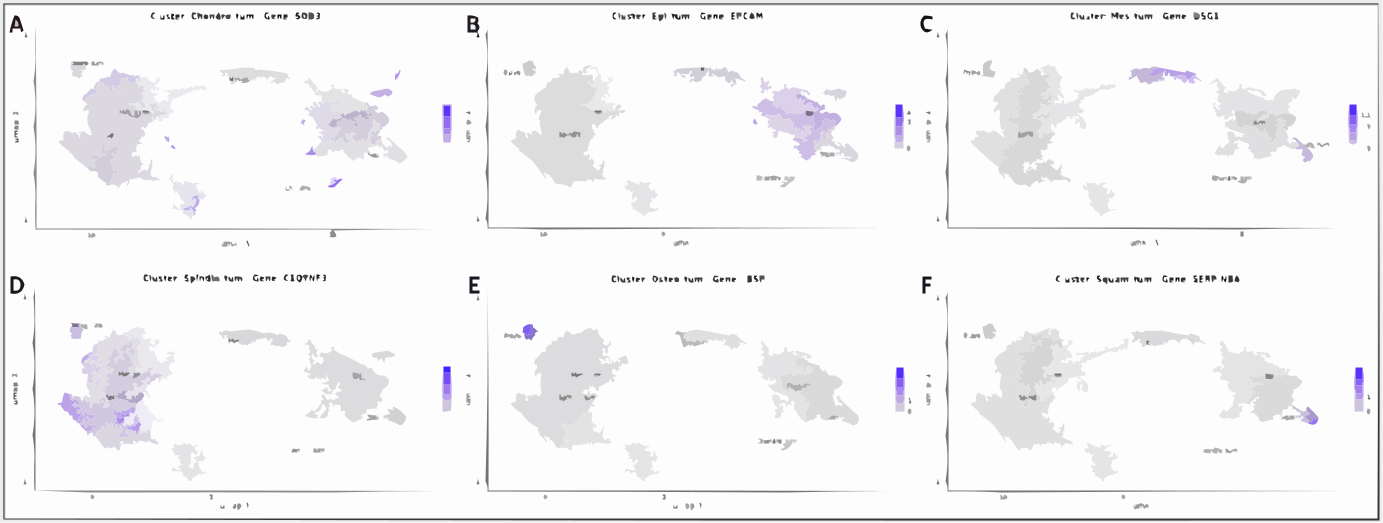
\includegraphics[width=\linewidth, height=0.6\textheight, keepaspectratio]{../Figures/Sans_légendes/Fig4.png}
    \caption[\textbf{Figure 4 : Visualisation de l’expression génique par cluster sur la projection UMAP.}]{\footnotesize \textbf{Visualisation de l’expression génique par cluster sur la projection UMAP.} La projection UMAP représente la distribution spatiale des archétypes. Chaque panneau montre la surexpression d’un marqueur phénotypique au sein des cellules tumorales chondroïdes \textbf{(A)}, tumorales épithéliales \textbf{(B)}, tumorales mésenchymateuses \textbf{(C)}, spindle-cell \textbf{(D)}, ostéosarcomatoïdes \textbf{(E)}, tumorales malpighiennes \textbf{(F)}, selon une échelle de couleur (du gris pour une faible expression au bleu pour une expression élevée).}
    \label{fig:fig4}
\end{figure}

Afin de mieux caractériser l’expression de ces marqueurs archétypiques, et leur pertinence pour notre problématique, nous avons analysé l’expression moyenne et le pourcentage exprimé dans les spots de cellules des meilleurs marqueurs, selon chacun des archétypes identifiés (\textbf{figure 5A}) ou la patiente d’origine (\textbf{figure 5B}). Nous pouvons constater sur la \textbf{figure 5A} que certains de ces marqueurs, comme le gène EPCAM, sont surexprimés dans la majorité des patientes présentant le type cellulaire étudié et faiblement exprimés dans les autres archétypes. De la même façon, le gène SPRR1B semble être un marqueur pertinent pour caractériser le archétypes des cellules tumorales malpighienne (\textbf{figure 5A}). Cependant, en regardant la \textbf{figure 5B}, on constate que ce marqueur n’est exprimé uniquement pour une seule patiente (MpBC8). Or la patiente MPBC3 présente aussi ce sous-type tumoral malpighien, et on ne retrouve pas d’expression de ce marqueur pour cette patiente. Ainsi donc, cela nous montre qu’au-delà d’une analyse sur la totalité des cellules de chaque archétype, il sera nécessaire de réaliser une analyse plus poussée pour garantir que les marqueurs les plus significatifs ne soient pas patient-dépendants.

\begin{figure}[H]
    \centering
    \includegraphics[width=\linewidth, height=0.6\textheight, keepaspectratio]{../Figures/Sans_légendes/Fig5_annot_tum.png}
    \caption[\textbf{Figure 5 : Profil d’expression des marqueurs par archétypes et par patients.}]{\footnotesize \textbf{Profil d’expression des marqueurs par archétypes et par patients.} Représentation DotPlot de l’expression normalisée des gènes marqueurs sélectionnés selon les archétypes spécifiques de chaque sous-types tumoraux \textbf{(A)} ou selon les patientes atteintes de MpBC \textbf{(B)}. La taille du point indique la proportion de cellules exprimant le gène, et la couleur du point reflète l’intensité moyenne d’expression normalisée.}
    \label{fig:fig5}
\end{figure}

\subsection{Analyse des altérations génomiques divergentes}

\subsubsection{Profils génomiques biphasiques}

\paragraph{Réduction par cytobande}

Pour obtenir le profil de CNA (\textit{Copy Number Alteration}) par patiente, nous avons utilisé le package R InferCNVPlus. Les résultats fournis par ce package se présentent sous la forme de matrices de scores CNA relatifs normalisés par échantillon : -1 pour la perte de matériel génétique maximale, +1 pour le gain maximal, et 0 pour le nombre de copies médian. Chaque ligne correspond à un spot et chaque colonne correspond à un gène. Dans notre analyse nous n’avons pas interprété directement les matrices brutes d’InferCNVPlus. Pour chaque patiente, nous avons plutôt analysé le profil CNA par compartiment tumoral (en faisant la médiane des scores par spot du même compartiment) et par cytobande (en faisant la médiane des scores par gène d’une même cytobande). Cela nous a permis d’obtenir la heatmap représenté en \textbf{figure 6}. On constate que les profils CNA des compartiments tumoraux appariés de chaque échantillon sont similaires pour la majorité des patientes et qu’on n’observe pas (ou peu) d’altérations du nombre de copie divergentes entre compartiment appariés.

\begin{figure}[H]
    \centering
    \includegraphics[width=\linewidth, height=0.6\textheight, keepaspectratio]{../Figures/Sans_légendes/Heatmap_all.png}
    \caption[\textbf{Figure 6 : Heatmap des résultats InferCNVPlus pour toutes les patientes.}]{\footnotesize \textbf{Heatmap des résultats InferCNVPlus pour toutes les patientes.} Les scores CNA médian par cytobande sont montré pour chaque compartiment tumoraux au sein de chaque patiente. Les compartiments tumoraux appariés dans les échantillons MpBC présentent des profils CNA similaires.}
    \label{fig:fig6}
\end{figure}

\paragraph{Normalisation intra-patiente et inter-compartiments.}

Nous travaillons ici avec des spots composés de plusieurs cellules, et donc avec une résolution supra-cellulaire. De plus il est important de noter que les spots peuvent présenter des profondeurs de séquençage différentes, en particulier selon le sous-type tumoral considéré. Nous avons donc procédé à une étape de normalisation afin de corriger les scores CNA des spots entre eux, à l’aide d’un facteur d’ajustement basé sur le rapport des scores CNA extrêmes entre les 2 tissus (voir Méthodes). Par exemple, pour la patiente MpBC9, le tissu tumoral épithélial présentait la plus forte amplification (\textbf{figure 7A}, chromosome 8), à laquelle le tissu tumoral chondroïde a été ajusté (\textbf{figure 7B}). La même correction a été appliquée pour les délétions (scores CNA < 0). Enfin, afin de faciliter la visualisation, les scores ont été renormalisés pour couvrir une échelle de -1 à 1, comme le signal InferCNVPlus initial. Cette normalisation a donc permis de faire coïncider les extremums des scores de délétion et d’amplification entre les différents compartiments tumoraux et de limiter les biais dus aux différences de profondeurs de séquençage et composition entre les différents compartiments. Par exemple, l’altération divergente du bras 8q avant normalisation (\textbf{figure 7A}) est complètement corrigée après ajustement (\textbf{figure 7B}). En revanche, d’autres différences, comme sur le bras 13q, persistent même après normalisation. En conclusion, cette normalisation a permis de corriger le signal de divergence entre CNA des compartiments appariés, pour garantir qu’ils n’étaient pas dûs à des différences d’abondance d’ARN ou de cellules.

\begin{figure}[H]
    \centering
    \includegraphics[width=\linewidth, height=0.6\textheight, keepaspectratio]{../Figures/Sans_légendes/Fig7_remix.png}
    \caption[\textbf{Figure 7 : Représentation des scores CNA obtenus avec InferCNVPlus, avant \textbf{(A)} et après normalisation \textbf{(B)}, en fonction des cytobandes mineures pour chaque chromosome du génome.}]{\footnotesize \textbf{Représentation des scores CNA obtenus avec InferCNVPlus, avant \textbf{(A)} et après normalisation \textbf{(B)}, en fonction des cytobandes mineures pour chaque chromosome du génome.} La ligne verticale en pointillé indique la position du centromère pour chaque chromosome. Les couleurs des courbes correspondent aux deux sous-types tumoraux comparés chez le patient MpBC9 (chondroïde tumorale en violet et épithélial tumorale en vert). Les scores CNA s’étendent de -1 à 0 (délétion) et de 0 à 1 (amplification).}
    \label{fig:fig7}
\end{figure}

\subsubsection{Identification des altérations divergentes entre compartiments appariés}

\paragraph{Test par bras chromosomique}

Afin d’identifier les altérations génomiques divergentes entre les compartiments appariés de chaque tumeur, nous avons testé si la distribution des différences de scores CNA entre compartiments pour un bras chromosomique donné, était significativement différente des différences dans les autres cytobandes. Les p-values obtenues lors des tests ont été corrigées, et considérées comme significatives lorsque la probabilité de commettre une erreur était très faible ($\alpha$=0.001). En plus de ce seuil alpha, une deuxième métrique plus représentative la taille de l’effet a été utilisée, à savoir la différence médiane entre les compartiments pour chaque bras chromosomique (voir Méthodes). La \textbf{figure 8} permet de représenter les bras chromosomiques significatifs par patiente sous forme d’un VolcanoPlot. La droite horizontale en pointillé indique le seuil de significativité ($\alpha$=0.001), tandis que les droites verticales en pointillé délimitent les seuils définissant une forte différence absolue de score entre compartiments. Par exemple, le bras chromosomique le plus significativement délété et avec la plus grande différence entre les compartiments tumoraux correspond au bras Xq chez la patiente MpBC16. Toutefois, bien que certains bras chromosomiques présentent des altérations divergentes significatives entre compartiment tumoraux, nous pouvons voir que cela ne concerne que quelques patientes uniquement.

\begin{figure}[H]
    \centering
    \includegraphics[width=\linewidth, height=0.6\textheight, keepaspectratio]{../Figures/Sans_légendes/Volcano.png}
    \caption[\textbf{Figure 8 : Volcano Plot des altérations CNA divergentes entre compartiments tumoraux appariés.}]{\footnotesize \textbf{Volcano Plot des altérations CNA divergentes entre compartiments tumoraux appariés.} Pour chaque patiente, les bras chromosomiques sont représentés selon la p-value ajustée (correction de Bonferroni, seuil $\alpha$ = 0,001) et la différence absolue de score CNA entre compartiments (seuil $\ge$ 0,27). Seules quelques patientes présentent des altérations significatives.}
    \label{fig:fig8}
\end{figure}

Enfin, afin de d’investiguer plus en détail les bras chromosomiques significativement divergents, nous avons représenté la corrélation des scores CNA par cytobandes pour chacun des compartiments tumoraux appariés de chaque échantillon. Un exemple des résultats pour les patientes MpBC9 et MpBC15 sont représentés sur la \textbf{Figure 9}. Chaque point représente le score normalisé obtenu pour chaque cytobande. Les cytobandes appartenant au bras retrouvé comme significatif par le test statistique ont été colorées en rouge. On constate que pour le bras chromosomique 13q chez MpBC9 (\textbf{figure 9A}) et MpBC15 (\textbf{figure 9B}), les cytobandes appartenant à ces bras sont outliers par rapport aux autres cytobandes. La \textbf{figure 9C} illustre ces altérations divergentes significatives sur le profil CNA. L’encadré rouge montre l’emplacement du bras chromosomique significativement divergent au sein du profil CNA. Pour conclure, cette figure montre que nous retrouvons quelques rares cas d’altération divergentes entre les compartiments tumoraux appariés.

\begin{figure}[H]
    \centering
    \includegraphics[width=\linewidth, height=0.6\textheight, keepaspectratio]{../Figures/Sans_légendes/Corrplot_remix.png}
    \caption[\textbf{Figure 9 : Analyse de la corrélation des scores CNA entre les deux sous-types tumoraux du patient MpBC9 et MpBC15.}]{\footnotesize \textbf{Analyse de la corrélation des scores CNA entre les deux sous-types tumoraux du patient MpBC9 et MpBC15.} Représentation de la corrélation entre les scores CNA du tissu tumoral chondroïde (en ordonnée) et épithélial tumoral (en abscisse) pour les patientes MpBC9 \textbf{(A)} et MpBC15 \textbf{(B)}. Chaque point correspond au score d’une cytobande mineure du bras chromosomique 13q. Les points rouges indiquent les cytobandes situées sur les bras chromosomiques significatifs. La ligne noire pleine représente une corrélation parfaite entre les scores CNA (droite d’identité), tandis que la ligne pointillée bleue indique la droite de régression linéaire ajustée au nuage de points. Les cytobandes des bras significatifs apparaissent comme des outliers, s’éloignant nettement de la droite d’identité. On retrouve ces altérations divergentes sur le profil CNA \textbf{(C)}.}
    \label{fig:fig9}
\end{figure}





\newpage






%% --- Discussions ---

\section{Discussion}

Les spots de la technologie Visium ont une taille d’environ 55µm et contiennent en moyenne 10 cellules. Bien que cette technologie permette d’allier l’information du séquençage transcriptomique à l’organisation spatiale du tissu, ce qui n’est pas possible par analyse \textit{bulk} ou \textit{single-cell}, cette pluralité des cellules par spot comporte certaines limitations. Cela peut en effet diluer le signal tumoral si les spots considérés comme tumoraux contiennent aussi des cellules normales. Dans notre projet, où un échantillon contient plusieurs sous-types tumoraux, cela peut mener à des « contaminations » locales très difficiles à éliminer, et à un bruit de fond pénalisant la précision des analyses transcriptomiques. Cela complique l’attribution précise d’un signal à un sous-type tumoral spécifique, et se traduit donc par un positionnement parfois diffus des spots dans l’espace vectoriel de la PCA et les projections UMAP. Il est par exemple difficile de définir une frontière exacte entre les différents sous-types mésenchymateux, fusiformes ou chondroïdes, produisant souvent de la matrice extracellulaire. Le signal transcriptomique issu de cette matrice peut artificiellement accroître les similitudes entre ces sous-types et les différents clusters se superposent entre eux. \\
Une solution serait d’utiliser une technique de déconvolution, permettant de connaitre la composition cellulaire d’un spot et ainsi de corriger le signal pour déterminer les transcrits provenant des cellules d’intérêt uniquement. Des travaux précédents au sein de l’équipe ont déjà montré que des outils tels que RCTD (Robust Cell Type Decomposition) \cite{Cable2022} sont assez puissants pour la déconvolution de spots Visium. Cependant, l’utilisation d’une déconvolution nécessite de comparer le profil transcriptomique de chaque spot aux profils transcriptomiques de référence caractéristiques de chaque type cellulaire. Or il n’existe actuellement aucun atlas transcriptomique de référence spécifique des différents sous-types tumoraux des MpBC. \\

Dans nos analyses, certains marqueurs phénotypiques identifiés montrent que nous arrivons en partie à capturer un signal biologique pertinent pour représenter certains sous-types tumoraux. Par exemple les marqueurs EPCAM et CD24 identifiés dans l’archétype correspondant aux cellules tumorales épithéliales, sont des marqueurs types des cellules épithéliales mammaires. De la même manière, le marqueur IBSP identifié pour le sous-type osteo-sarcomatoïde correspond à une glycoprotéine de la matrice extracellulaire osseuse, tandis que le marqueur SERPINB4 identifié pour le sous-type épidermoïde correspond à un antigène connus des cancers kératinocytaires. Toutefois, on constate que pour le moment, de nombreux marqueurs identifiés par DGEA sont encore souvent soit trop peu spécifiques d’un seul sous-type, soit pas assez représentatifs de tous les patients d’un sous-type. Cela suggère donc qu’il sera nécessaire d’obtenir une meilleure précision par la suite. \\

Les limites de la technologie Visium peuvent également biaiser l’inférence du score CNA prédit par InferCNVPlus. L’estimation de ces scores CNA repose sur l’augmentation ou la réduction d’expression génique sur une portion de génome pour détecter des altérations du nombre de copies génomiques. Or, l’incorporation de cellules non tumorales peut « diluer » le signal tumoral, car les cellules non tumorales ont un profil génomique parfaitement diploïde. De plus, dans notre projet, tous les spots n’auront pas la même densité cellulaire ce qui dépendra du sous-type tumoral considéré. Par exemple, un spot contenant des cellules tumorales chondroïdes, isolées au sein de larges zones de matrice cartilagineuse, présentera une densité cellulaire plutôt faible. A l’inverse, un spot capturant des cellules épithéliales, de nature jointives et adhérentes entre elles, sera plus densément peuplé. En conséquence, le score d’altération du nombre de copie peut s’en retrouver sous-estimé pour certains spots, faussant l’analyse. Enfin, cette technologie basée sur l’ARN est inadaptée à la segmentation précise et la quantification exact du nombre des CNA somatiques du cancer. Des approches ADN pourraient permettre de mieux caractériser l’évolution génétique entre les compartiments différents des MpBC mixtes.\\

Nous avons pu observer que les profils CNA des différents compartiments tumoraux appariés étaient très similaires, suggérant fortement une origine commune. Nos analyses ont tout de même permis d’identifier des altérations divergentes entre compartiments tumoraux appariés affectant des bras chromosomiques entiers. Cela suggère l’existence d’une relation clonale dans ces quelques cas, où l’un des 2 sous-types a pour origine une cellule de l’autre. Parmi tous les CNA divergents identifiées, la véritable question est de savoir si ces altérations génomiques sont des passagères, ou des drivers de la transdifférenciation dans les MpBC. Les mutations passagères correspondent à des altérations sans réel rôle fonctionnel, mais dont la fréquence élevée permet de suivre l’évolution graduelle du génome. En revanche, un CNA driver correspond à un changement du nombre de copie de gène spécifique contribuant activement à une progression de la tumeur (ici, la transdifférenciation). A l’avenir, une plus grande cohorte pourrait permettre d’identifier des CNA récurrents dans certaines transdifférenciations, et donc plus à même d’être des drivers.\\

Ce travail s’inscrit dans un cadre plus large d’un consortium de recherche national sur le carcinome mammaire métaplasique, comprenant le CLB à Lyon, l’institut Bergonié à Bordeaux, le Centre de Recherche en Cancérologie et Immunologie à Nantes et l’Institut Curie à Paris. Il regroupe de nombreux chercheurs et praticiens cliniques, et centralise la collecte des données cliniques et omiques des patientes atteintes de MpBC en France. A ce jour, on dénombre 140 tumeurs de MpBC réunies grâce à ce projet, fournissant aux chercheurs un pool de données importantes pour développer la recherche de nouvelles thérapies et marqueurs de diagnostic afin d’améliorer la prise en charge des patientes atteintes de ces cancers métaplastiques \cite{bergonie}. Cela représente une opportunité d’enrichir notre dataset avec de nouveaux échantillons, et donc d’augmenter la représentation de chaque sous-type et la puissance statistique dans nos analyses. Cela permettra ainsi de pallier à certains manques de cette étude préliminaire.\\

Un des objectifs de ce projet est de trouver des marqueurs d’expression caractéristiques et spécifiques de chacun des sous-types tumoraux dans les MpBC. Nous n’avons donc, aujourd’hui pas ou peu, de piste sur lesquels nous reposer pour identifier des marqueurs fiables. De fait, devant la grande diversité et le nombre important de gènes potentiels identifiés durant l’analyse DGEA des marqueurs d’expression de chaque sous-type tumoral, il est complexe de savoir quels marqueurs sont pertinents. Dans notre étude, l’utilisation de logiciel comme SCENIC \cite{Aibar2017SCENIC} pourrait aider à réduire le nombre de piste d’intérêt, tout en analysant mieux les gènes régulateurs pertinents mais qui pourraient être faiblement exprimés. Ainsi nous pourrions expliquer les profils d’expressions et de transdifférenciation observés dans chaque sous-type, selon les facteurs de transcription exprimés et les potentielles voies de signalisation dérégulées dans chaque sous-type de MpBC.\\

Afin de corriger la résolution insuffisante des spots Visium, une solution évoquée précédemment serait de compléter l’analyse par une étape de déconvolution du signal transcriptomique pour chaque spot. Cela permettrait d’identifier ainsi les différents types cellulaires et leurs proportions au sein des spots. Pour réaliser cela, nous prévoyons de compléter les données spatiales avec des données de scRNAseq, permettant l’analyse ARN des cellules uniques pour chaque échantillon. Plus précisément cela est envisagé par single-nuclei RNAseq (séquençage des noyaux uniques), plus adapté aux échantillons fixés en paraffine (FFPE). Ces données transcriptomiques générées à l’échelle de la cellule unique permettront de créer un profil transcriptomique spécifique pour chaque sous-type cellulaire, auquel nous pourrons nous rapporter lors de l’étape de déconvolution des spots. Cela permettra à la fois de mieux évaluer la composante micro-environnementale des différents compartiments, et des éventuelles différences qui les caractérisent, mais aussi d’identifier des marqueurs sur des données « pures » au niveau de chaque type cellulaire, et donc plus spécifiques.\\

Dans le but d’explorer en profondeur les dynamiques évolutives des échantillons biphasiques MpBC, des microdissections par capture laser vont être effectuées afin de déterminer les caractéristiques génétiques uniques des deux compartiments de chaque échantillon. L’ADN spécifique à chaque compartiment pourra être extrait et les déterminants génétiques somatiques, tels que les CNA mais aussi désormais les mutations ponctuelles, seront analysés par séquençage d’exome entier. A l’aide de ces analyses basées sur de l’ADN plus adapté que l’ARN, on pourra ainsi valider plus précisément les CNA identifiés avec mon analyse préliminaire, mais aussi de suivre plus précisément les probables relations clonales entre compartiment appariés.  \\

Les microdissections de chaque compartiment tumoral pourront également permettre une analyse épigénétique de chaque sous-type. Nous pourrons révéler les gènes suppresseurs de tumeurs hyperméthylés et inactivés par silencing, ou au contraire des oncogènes hypométhylés favorisant la prolifération et la survie, et l’instabilité génomique des cellules tumorales. Ce type d’analyse est particulièrement intéressante dans notre projet car il a été montré à de nombreuses reprises dans la littérature scientifique que certaines modifications épigénétiques sont à l’origine d’un remodelage de l’identité des cellules tumorales \cite{Gronbaek2007Epigenetic}.\\

De plus, il est aujourd’hui connu que de nombreuses cellules immunitaires (lymphocytes T CD4, CD8, macrophages) et non immunitaires (CAF (Cancer Associated Fibroblast)) jouent un rôle prépondérant dans la constitution de niches biologiques au sein du tissu tumoral, pouvant réguler la trajectoire évolutive des populations tumorales \cite{fondationarc2020caf}. Grâce à la déconvolution des spots Visium, nous pourrons ainsi évaluer la composition du microenvironnement tumoral pour chaque compartiments transdifférenciés et déterminer si des facteurs externes pourraient être à l’origine de la transdifférenciation en un sous-type spécifique. L’identification de paires ligand-récepteurs permettra de révéler de potentielles interactions entre les cellules transdifférenciés et les cellules du micro-environnement. La spatialisation du signal dans les données de transcriptomique spatiale permettra d’identifier d’éventuels patterns d’expression ségréguée, pour déterminer si ces ligands, récepteurs et les voies qu’ils régulent présentent une expression différente entre l’environnement immédiat, la bordure et le cœur des compartiments tumoraux.\\

Finalement, chacun des biomarqueurs identifiés comme spécifiques de chaque sous-type fera l’objet d’une validation Immunohistochimique (IHC) dans la cohorte MpBC indépendante de l’Institut Curie, afin d’estimer leur pertinence pour le diagnostic moléculaire. Enfin, les biobanques d’organoïdes et xénogreffes dérivées de patientes MpBC par les collaborateurs de l’équipe permettront d’étudier le rôle des biomarqueurs et des voies identifiées, via des perturbations génétiques et pharmacologiques. 





\newpage


\section{Conclusions}

Les objectifs de ce stage étaient, dans un premier temps, d’explorer les données transcriptomiques spatiales des carcinomes mammaires métaplasiques générées avec la technologie Visium. Cette première approche visait notamment à définir des gènes impliqués dans la transdifférenciation, et spécifiques de chaque sous-type tumoraux. Puis, via des analyses d’altérations du nombre de copie, d’identifier des altérations génétiques qui pourraient être à l’origine des transdifférenciations entre les compartiments tumoraux.\\
A travers l’analyse de 16 premiers échantillons MpBC, j’ai pu identifier des marqueurs phénotypiques prometteurs pour certains sous-types tumoraux. Toutefois des analyses plus poussées permettront de valider leur pertinence, et d’identifier des marqueurs spécifiques pour tous les sous-types. Mes analyses suggèrent de plus que les 2 compartiments de chaque tumeur analysée ont la même cellule d’origine. J’ai pu identifier de rares altérations suggérant une évolution clonale entre les compartiments, mais cela ne concerne qu’une partie des échantillons, suggérant que les CNAs ne sont en général pas la cause des transdifférenciations observées.\\
Bien que certaines limitations, liées à la résolution spatiale des spots de la technologie Visium, limitent encore la portée de mes analyses, ces premiers résultats constituent tout de même une base solide et encourageante pour la suite du projet, nous permettant d’orienter nos prochaines recherches.\\
Ce travail m’a également permis de consolider grandement mes connaissances dans les analyses de transcriptomique spatiale et des outils associés, avec à la fois des applications phénotypiques et génomiques.


\newpage

\bibliographystyle{unsrt}
\bibliography{references}

\end{document}
